\documentclass[11pt,a4paper]{article}

% ============================================================================
% Packages
% ============================================================================
\usepackage[utf8]{inputenc}
\usepackage[T1]{fontenc}
\usepackage{lmodern}
\usepackage{amsmath,amssymb,amsfonts,amsthm}
\usepackage{graphicx}
\usepackage[dvipsnames,svgnames,x11names]{xcolor}
\usepackage{geometry}
\usepackage{booktabs}
\usepackage{fancyhdr}
\usepackage{hyperref}
\usepackage{tikz}
\usepackage{pgfplots}
\usepackage{float}
\usepackage{enumitem}
\usepackage{caption}
\usepackage{subcaption}
\usepackage{tabularx}
\usepackage{mathtools}
\usepackage{tcolorbox}
\usepackage{titlesec}
\usepackage{parskip}
\usepackage{epigraph}

\usetikzlibrary{arrows.meta,positioning,calc,decorations.pathmorphing,backgrounds,fit,shapes.geometric}
\pgfplotsset{compat=1.18}

\geometry{margin=2.5cm,top=2.8cm,bottom=2.8cm}

\newtheorem{theorem}{Theorem}[section]
\newtheorem{lemma}[theorem]{Lemma}
\newtheorem{definition}[theorem]{Definition}
\newtheorem{remark}[theorem]{Remark}

\tcbuselibrary{skins,breakable}

% ============================================================================
% Colors
% ============================================================================
\definecolor{quantumcyan}{HTML}{00D4FF}
\definecolor{quantumpurple}{HTML}{8B5CF6}
\definecolor{quantumgreen}{HTML}{10B981}
\definecolor{sectionblue}{HTML}{2563EB}
\definecolor{measured}{HTML}{059669}
\definecolor{hardcoded}{HTML}{D97706}
\definecolor{theoretical}{HTML}{7C3AED}
\definecolor{chalkboard}{HTML}{1A2332}

% Custom environments
\newtcolorbox{honesty}{
    colback=orange!5, colframe=orange!70!black,
    fonttitle=\bfseries\small, title={Data Honesty Note}, breakable
}

\newtcolorbox{blackboard}[1][]{
    colback=chalkboard!95!black, colframe=chalkboard,
    coltext=white, fonttitle=\bfseries\color{quantumcyan},
    title={#1}, breakable, arc=2mm
}

\newtcolorbox{susskindbox}[1][]{
    colback=blue!3, colframe=sectionblue!60,
    fonttitle=\bfseries\small\color{sectionblue},
    title={#1}, breakable
}

% ============================================================================
% Hyperref
% ============================================================================
\hypersetup{
    colorlinks=true, linkcolor=sectionblue, citecolor=quantumpurple, urlcolor=quantumcyan,
    pdftitle={The Theoretical Minimum for Blockchain Consensus},
    pdfauthor={Q-NarwhalKnight Research},
}

% ============================================================================
% Header/Footer
% ============================================================================
\pagestyle{fancy}
\fancyhf{}
\fancyhead[L]{\small\textcolor{gray}{The Theoretical Minimum for Blockchain Consensus}}
\fancyhead[R]{\small\textcolor{gray}{v4 --- April 2026}}
\fancyfoot[C]{\small\textcolor{gray}{\thepage}}
\renewcommand{\headrulewidth}{0.4pt}

\setlength{\epigraphwidth}{0.75\textwidth}

% ============================================================================
% Title
% ============================================================================
\title{%
\vspace{-1cm}
{\LARGE\textbf{The Theoretical Minimum\\for Blockchain Consensus}}\\[0.4cm]
{\large A Statistical Mechanics Framework for DAG-Knight,\\Explained from First Principles}\\[0.4cm]
{\normalsize\textcolor{gray}{With honest accounting of what we measure, what we assume,\\and what we don't know yet}}\\[0.3cm]
{\small\textcolor{sectionblue}{Revised after peer review by DeepSeek, ChatGPT, and Gemma~4}}
}

\author{%
\textbf{Q-NarwhalKnight Research}\\
\texttt{research@quillon.xyz}\\[0.2cm]
{\small Network: \texttt{mainnet-genesis} $\mid$ v10.2.8 $\mid$ 14,329,651 blocks $\mid$ 12 peers $\mid$ 47.9 days uptime}
}

\date{April 11, 2026 --- v4}

\begin{document}
\maketitle

\epigraph{``The best thing about physics is that it tells you when you're wrong. The worst thing about physics-inspired analogies is that they never do.''}{---Adapted, in the spirit of Susskind}

% ============================================================================
% Abstract
% ============================================================================
\begin{abstract}
We present an observability framework for DAG-Knight blockchain consensus that uses the language of statistical mechanics---Hamiltonians, temperature, phase diagrams, entropy, and diffusion---to organize network diagnostics into a coherent, quantitative picture. We are explicit about the epistemological status of every claim: one theorem is proven (the Ground State Correspondence), several formulas are testable quantitative models, and the rest is structural analogy. We validate against 14.3 million blocks on a live mainnet, present simulated stress scenarios, and catalog every measurement gap where hardcoded placeholders replace real data. The paper is written in an expository style inspired by Susskind's \emph{Theoretical Minimum}: we explain what each formula means, why we chose it, where it comes from, and where it fails. This is an engineering contribution dressed in physics notation---not a physics contribution. The physics notation is useful because it gives us additive decomposition (Hamiltonian), a single stress scalar (temperature), a visual operating envelope (phase diagram), and an information-theoretic measure of ambiguity (entropy). We use these tools honestly and invite the reader to hold us to that standard.

In v4, we introduce two information-theoretic enhancements motivated by recent work in quantum gravity (Harlow, Usatyuk \& Zhao, 2025) and computational universe theory (Lloyd, 2006): an \emph{observer coverage factor} that flags nodes with limited network visibility, and a \emph{block commitment depth} that measures finality irreversibility. Both quantities are measurable from existing data structures and integrate with the $K$-gauge. These additions address a blind spot identified in v3: the gauge's inability to detect adversarial behavior that maintains normal operational metrics.
\end{abstract}

\tableofcontents
\newpage

% ============================================================================
% PART I: WHY PHYSICS NOTATION?
% ============================================================================
\part{Why Physics Notation for a Blockchain?}

% ============================================================================
% 1. The Problem
% ============================================================================
\section{The Problem: What Does ``Healthy'' Mean?}

Imagine you're a node operator. You stare at a dashboard that says:

\begin{quote}
Height: 14,329,651 \quad Peers: 12 \quad Blocks per second: 3.46
\end{quote}

You nod. ``Looks fine.''

But wait---\emph{does} it? What if half the network disagrees on which block came first? What if you're one adversarial peer away from losing consensus? What if the ordering of the last 1000 blocks could be flipped with a little extra hashrate?

The dashboard doesn't tell you any of that. It's like a car speedometer that shows only RPM but not engine temperature, oil pressure, or whether you're about to drive off a cliff.

A network can produce blocks and still be:

\begin{itemize}
    \item \textbf{Slow to converge} --- nodes disagree on block ordering for too long.
    \item \textbf{Close to a security boundary} --- one more adversarial peer and consensus breaks.
    \item \textbf{Producing ambiguous orderings} --- multiple valid ways to order concurrent blocks.
    \item \textbf{Under subtle attack} --- an adversary maintaining ``normal'' metrics while slowly poisoning the DAG.
\end{itemize}

We need a dashboard for \emph{consensus health}. And we need it to be:

\begin{itemize}
    \item \textbf{Decomposable} --- you can see \emph{why} the network is stressed (too many concurrent blocks? high latency? adversarial activity?).
    \item \textbf{Quantitative} --- a single number that says ``stable'' or ``warning'' or ``emergency.''
    \item \textbf{Verifiable} --- other nodes can check your health report without you revealing your internal secrets.
\end{itemize}

That's what we build in this paper. And we're going to borrow a very powerful toolkit from physics: \textbf{statistical mechanics}.

Now, before you roll your eyes: I am \emph{not} saying the blockchain is a physical system. It's not made of atoms, it doesn't have a temperature in Kelvin, and it doesn't undergo Bose--Einstein condensation. But physicists have spent 150 years learning how to decompose complex systems into additive energy terms, define a single ``temperature'' that captures disorder, and draw phase diagrams that show where the system works and where it breaks.

Those mathematical structures are \emph{exactly} what we need for consensus. So we're going to steal them. Respectfully.

% ============================================================================
% 2. What We're Not Claiming
% ============================================================================
\section{What We Are \emph{Not} Claiming}

Before we write a single equation, let's be clear about the epistemological status of this work. We classify every claim at one of three levels:

\begin{susskindbox}[Three Levels of Claims]
\begin{enumerate}
    \item \textbf{Exact Theorem} (\textcolor{measured}{$\blacksquare$}): A proven mathematical statement with explicit assumptions. We have exactly one of these---the Ground State Theorem (Section~\ref{sec:groundstate}), which proves that the Hamiltonian's minimum corresponds to the PHANTOM algorithm's output.

    \item \textbf{Quantitative Model} (\textcolor{hardcoded}{$\blacksquare$}): A formula that makes testable predictions. The effective temperature $T_{\text{eff}}$, the critical threshold $\kappa_c$, and the diffusion model are at this level. They could be \emph{wrong}---but they're wrong in a falsifiable way.

    \item \textbf{Structural Analogy} (\textcolor{theoretical}{$\blacksquare$}): Conceptual vocabulary borrowed from physics for intuition. ``Temperature,'' ``entropy,'' and ``phase transition'' are used at this level. They help organize thinking but don't imply the blockchain exhibits thermodynamic phenomena.
\end{enumerate}
\end{susskindbox}

The previous version of this paper (v1) was reviewed by DeepSeek and ChatGPT. Both rejected it, correctly identifying that we had blurred the lines between these levels---presenting structural analogies as if they were exact theorems, and hardcoded constants as if they were live measurements. This version fixes that.

\subsection{An Analogy for the Analogy}

Think of it this way. When economists talk about ``market temperature'' or ``economic entropy,'' nobody believes the stock market is literally at 300 Kelvin. But the language is useful: high ``temperature'' means high volatility; low ``entropy'' means concentrated positions. The math of statistical mechanics---Boltzmann distributions, partition functions, free energy---turns out to be the right formalism for many systems that have nothing to do with atoms.

We're doing the same thing for consensus. The DAG is not a spin system. But it \emph{does} have a well-defined configuration space (the set of all valid orderings), an objective function (the PHANTOM blue-score), and a noise parameter (network latency and adversarial fraction). That's enough structure to borrow the vocabulary.

% ============================================================================
% 3. Data Provenance
% ============================================================================
\section{Data Provenance: What We Actually Measure}
\label{sec:provenance}

This is the most important section of the paper. Every quantity we use falls into one of four categories:

\begin{table}[H]
\centering
\caption{Complete data provenance for all quantities in this paper.}
\label{tab:provenance}
\small
\begin{tabular}{@{}p{3.5cm}lcp{5cm}@{}}
\toprule
\textbf{Quantity} & \textbf{Symbol} & \textbf{Src} & \textbf{Details} \\
\midrule
\multicolumn{4}{l}{\textbf{\textcolor{measured}{MEASURED from live network state}}} \\
\midrule
Block height & $|V|$ & \textcolor{measured}{M} & Atomic counter, updated every block \\
Peer count & $n$ & \textcolor{measured}{M} & libp2p connection count \\
Block rate & $\Lambda$ & \textcolor{measured}{M} & $|V|$ / (now $-$ genesis\_timestamp) \\
Mining rejection ratio & $r$ & \textcolor{measured}{M} & submitted/accepted atomic counters \\
Traffic asymmetry & $\alpha$ & \textcolor{measured}{M} & P2P byte counters in/out \\
Peer churn & $c$ & \textcolor{measured}{M} & Peer count delta per window \\
Sync divergence & $\sigma_s$ & \textcolor{measured}{M} & $|h_{\text{net}} - h_{\text{local}}|/h_{\text{net}}$ \\
Block rate deviation & $\sigma_\Lambda$ & \textcolor{measured}{M} & $|\Lambda - \Lambda_{\text{target}}|$ \\
\midrule
\multicolumn{4}{l}{\textbf{\textcolor{sectionblue}{PROTOCOL CONSTANTS (correctly fixed by design)}}} \\
\midrule
DAG-Knight $\kappa$ & $\kappa$ & \textcolor{sectionblue}{P} & Protocol parameter = 18 \\
Security levels & --- & \textcolor{sectionblue}{P} & Dilithium-5: 256-bit, Kyber-1024: 200-bit \\
Dandelion++ stem & --- & \textcolor{sectionblue}{P} & 4 hops \\
K-gauge window & $\tau$ & \textcolor{sectionblue}{P} & 60 seconds \\
\midrule
\multicolumn{4}{l}{\textbf{\textcolor{hardcoded}{HARDCODED PLACEHOLDERS (should be measured, aren't)}}} \\
\midrule
Propagation delay & $\delta$ & \textcolor{hardcoded}{H} & Hardcoded 0.2s. Per-peer RTT exists in \texttt{peer\_latency.rs} but is not wired \\
Mesh degree & $d$ & \textcolor{hardcoded}{H} & Hardcoded 8. Actual mesh degree not tracked \\
Byzantine fraction & $f/n$ & \textcolor{hardcoded}{H} & Hardcoded 0.0. No estimation from peer behavior \\
Blue density & $\varphi$ & \textcolor{hardcoded}{H} & $= 1 - f/n = 1.0$ (computed from hardcoded $f/n$) \\
Anticone size & $\bar{a}$ & \textcolor{hardcoded}{H} & Estimated as $2\delta\Lambda$. SIMD computation exists but not exported \\
\midrule
\multicolumn{4}{l}{\textbf{\textcolor{red}{NOT IMPLEMENTED (referenced in theory, no code)}}} \\
\midrule
Partition function & $\mathcal{Z}$ & \textcolor{red}{N} & Defined mathematically; not computed \\
Emission feedback & --- & \textcolor{red}{N} & Referenced in API response; no feedback loop exists \\
\midrule
\multicolumn{4}{l}{\textbf{\textcolor{sectionblue}{v4 ADDITIONS (information-theoretic enhancements)}}} \\
\midrule
Network size estimate & $n_{\text{total}}$ & \textcolor{hardcoded}{H} & Estimated from DHT peer discovery; not precisely measured \\
Commitment depth & $d_{\text{commit}}$ & M$^*$ & Descendant count per block; computable from DAG, not yet exported \\
Reorg depth bound & $D_{\text{reorg}}$ & \textcolor{hardcoded}{QM} & Derived from DAG-Knight security proof \\
Commitment weight & $\mu$ & \textcolor{hardcoded}{H} & Needs calibration against reorg events \\
Confirmation target & $\tau_{\text{confirm}}$ & P & Protocol constant, proposed = 100 blocks \\
Observer weight & $w_{\text{obs}}$ & P & Protocol constant, proposed = 1.0 \\
\bottomrule
\end{tabular}
\end{table}

\paragraph{Why publish with hardcoded values?} Because the framework is useful even with placeholders. The Hamiltonian decomposition tells you \emph{which dimensions} of health to monitor, even if some dimensions aren't fully instrumented yet. The $K$-gauge uses only measured inputs. And the phase diagram, even with hardcoded $\delta$ and $f/n$, correctly visualizes the \emph{structure} of the security margin.

But we owe the reader complete transparency about what's real and what's placeholder. That's what this table provides.

% ============================================================================
% PART II: THE HAMILTONIAN
% ============================================================================
\part{The Consensus Hamiltonian}

\section{What Is a Hamiltonian, and Why Do We Want One?}

In physics, the Hamiltonian $H$ is the total energy of a system. It's a function that takes a configuration---positions and momenta of all particles---and returns a single number. The magic is this: \textbf{the configuration that minimizes $H$ is the most stable one}---the ground state.

For a blockchain, the ``configuration'' is a total ordering of all blocks (respecting parent--child edges). The ``ground state'' is the consensus ordering---the one all honest nodes agree on.

So if we can write a Hamiltonian whose minimum is the \emph{right} ordering, then we can:

\begin{itemize}
    \item Measure how far the current ordering is from the ground state (energy gap).
    \item Define a ``temperature'' that quantifies how much randomness / disagreement exists.
    \item Find a phase transition---a critical value of some parameter where consensus breaks down.
    \item Compute entropy---how many different orderings are almost as good as the ground state.
\end{itemize}

That's the plan. We're going to define four energy terms, each penalizing a different kind of ``badness.'' Think of it like a report card with four grades: causality, ambiguity, honesty, and time-anchoring. The Hamiltonian is the weighted sum of all four.

\section{Configuration Space: What Are We Optimizing Over?}

\begin{definition}[Configuration Space]
Let $G = (\mathcal{V}, \mathcal{E})$ be the block DAG, where $\mathcal{V}$ is the set of blocks and $\mathcal{E}$ is the set of parent-child edges. A \emph{configuration} $\sigma$ is a total ordering of $\mathcal{V}$ that respects all edges in $\mathcal{E}$---i.e., if block $A$ is a parent of block $B$, then $A$ comes before $B$ in $\sigma$. The set of all valid configurations is $\Omega$, the set of \emph{linear extensions} of $G$.
\end{definition}

$|\Omega|$ can be enormous. For a DAG with $N$ blocks and average anticone size $\bar{a}$, the number of valid orderings is roughly $|\Omega| \approx \prod_{v} |\text{anticone}(v)|!$ (this is an approximation; the exact count is \#P-complete~\cite{brightwell}).

In Susskind's language: $\Omega$ is the phase space of the consensus system. Each configuration $\sigma \in \Omega$ is a ``microstate.'' The Hamiltonian assigns an energy to each microstate, and the ground state is the consensus ordering.

\section{The Four Energy Terms}

We decompose the Hamiltonian into four terms, each capturing a different dimension of ordering quality:

\begin{equation}
\boxed{H_{\text{DAG}}(\sigma) = H_p(\sigma) + H_a(\sigma) + H_b(\sigma) + H_{\text{VDF}}(\sigma)}
\label{eq:hamiltonian}
\end{equation}

Let's unpack each one in the style of a blackboard lecture.

\begin{figure}[H]
\centering
\includegraphics[width=0.95\textwidth]{fig_energy_landscape.png}
\caption{The consensus Hamiltonian energy landscape. The deep blue valley is the ground state---the PHANTOM consensus ordering. Surrounding hills and ridges represent disordered or adversarial orderings with higher energy. The dashed line shows the effective temperature $T_{\text{eff}} = 0.692$: thermal fluctuations (network noise, latency, concurrent blocks) can push the system up to this level, but cannot reach the high-energy adversarial peaks. The five energy terms are decomposed in the bar chart below: causality (green), ambiguity (orange), honesty (cyan), time-anchoring (purple), and the v4 addition---finality/commitment depth (gold).}
\label{fig:landscape}
\end{figure}

\subsection{Parent Energy: Respecting Causality}

\begin{blackboard}[Parent Energy $H_p$]
\begin{equation}
H_p(\sigma) = -J_p \sum_{(v_i, v_j) \in \mathcal{E}} \Theta(\sigma(v_j) - \sigma(v_i))
\end{equation}

\textbf{What it means:} For every parent-child pair $(v_i, v_j)$, check if the parent $v_i$ comes before the child $v_j$ in the ordering $\sigma$. If yes, contribute $0$ to the energy (correct). If no, contribute $+J_p$ (penalty).

\textbf{In practice:} $J_p = \infty$. The protocol \emph{rejects} blocks that violate causality. So $H_p = 0$ always, and we only consider orderings in $\Omega$ (linear extensions). This is analogous to a hard constraint in physics---like saying ``particles can't overlap.''

\textbf{On the live network:} $H_p = 0$ across all 14,329,651 blocks. This is not surprising---it's enforced by the protocol, not emergent.
\end{blackboard}

\subsection{Anticone Energy: The Cost of Ambiguity}

\begin{blackboard}[Anticone Energy $H_a$]
\begin{equation}
H_a(\sigma) = \lambda \sum_{v \in \mathcal{V}} \left(\frac{|\mathrm{anticone}(v)|}{\kappa}\right)^2
\end{equation}

\textbf{What it means:} The \emph{anticone} of a block $v$ is the set of blocks that are neither ancestors nor descendants of $v$---blocks that were created ``at the same time'' in the causal sense. If Alice and Bob both create a block before seeing each other's blocks, their blocks are in each other's anticone.

Large anticones mean ambiguity: there are many valid ways to order concurrent blocks, and the network might disagree. The quadratic penalty ensures that a few blocks with large anticones (potential attack vectors) contribute more energy than many blocks with small anticones.

\textbf{The $\kappa$ parameter:} The protocol parameter $\kappa = 18$ sets the ``tolerance''---anticone sizes up to $\kappa$ are expected and mildly penalized; sizes much larger than $\kappa$ are exponentially suppressed.

\textbf{Why quadratic?} Linear penalties would mean that distributing adversarial blocks evenly is equally costly as concentrating them. The quadratic penalty makes concentration (which is the more dangerous attack pattern) energetically expensive. This is analogous to a confining potential in physics.
\end{blackboard}

\begin{honesty}
On the live network, we \emph{estimate} the average anticone size as $\bar{a} = 2\delta\Lambda = 2 \times 0.2 \times 3.46 \approx 1.4$, rounded to 1. But $\delta = 0.2$s is hardcoded, and the actual SIMD-computed anticone sizes (which exist in \texttt{simd\_sets.rs}) are not exported to the observability endpoint. The true average anticone size on the live network is unknown to us.

This is the single most important measurement gap in the framework. Section~\ref{sec:limitations} proposes closing it.
\end{honesty}

\subsection{Blue Score: Rewarding Honest Blocks}

\begin{blackboard}[Blue Score Energy $H_b$]
\begin{equation}
H_b(\sigma) = -J_b \sum_{v \in \mathcal{V}} \mathbb{1}[\mathrm{blue}(v)] \cdot w(v)
\end{equation}

\textbf{What it means:} The PHANTOM/GhostDAG coloring algorithm classifies each block as ``blue'' (honest, well-connected) or ``red'' (potentially adversarial, poorly connected). A block is blue if its anticone size is bounded by $\kappa$---it doesn't conflict with too many other blocks.

Blue blocks get negative energy (favorable). The more blue blocks in the DAG, the lower the total energy, the more stable the consensus.

\textbf{The coloring algorithm:} PHANTOM finds the maximum-weight $\kappa$-cluster in the DAG's anticone graph. A $\kappa$-cluster is a set of blocks where every pair has anticone size $\leq \kappa$ relative to the cluster. This is an NP-hard problem in general, but GhostDAG provides a greedy approximation that runs in linear time.

\textbf{The blue density $\varphi$:} We define $\varphi = |B|/|V|$ (the fraction of blocks that are blue). In a healthy network with no adversaries and low latency, $\varphi \to 1.0$ (all blocks are blue). Under attack with $f/n$ adversarial nodes, $\varphi \to 1 - f/n$ (adversarial blocks are red).

$\varphi$ is the \emph{order parameter} of the system---the number that distinguishes the ordered phase (consensus, $\varphi \approx 1$) from the disordered phase (no consensus, $\varphi \to 0$). In physics, this is called a Landau order parameter, after Lev Landau who introduced the concept in the 1930s for classifying phase transitions.
\end{blackboard}

\begin{honesty}
The blue density $\varphi$ is currently hardcoded as $1 - f/n = 1.0$ because $f/n$ is hardcoded to 0. The DAG-Knight implementation \emph{does} compute blue/red classification internally (\texttt{ordering\_rules.rs}), but it does not export vertex color statistics to the observability endpoint.

Claiming $\varphi = 1.0$ from a hardcoded constant is circular reasoning. We know $\varphi$ should be close to 1.0 on an honest 12-peer network, but we cannot verify it without exporting the actual coloring.
\end{honesty}

\subsection{VDF Anchoring: The Cost of Time}

\begin{blackboard}[VDF Energy $H_{\text{VDF}}$]
\begin{equation}
H_{\text{VDF}}(\sigma) = -\sum_{v \in \mathcal{V}} \mathbb{1}[\mathrm{VDF}(v) \text{ valid}]
\end{equation}

\textbf{What it means:} A Verifiable Delay Function (VDF) is a cryptographic proof that a minimum amount of wall-clock time has passed. Each block carries a VDF proof, anchoring it to real time.

Why does this matter? Without VDF anchors, an adversary could pre-compute blocks and release them strategically (a ``selfish mining'' or ``time-warp'' attack). The VDF prevents this by requiring sequential computation that cannot be parallelized.

Each valid VDF proof contributes $-1$ to the energy. The more time-anchored blocks, the more stable the consensus.

\textbf{On the live network:} Every block has a valid VDF proof, so $H_{\text{VDF}} = -|V| = -14{,}329{,}651$. This is fully measured (we count blocks with valid proofs).
\end{blackboard}

\section{The Ground State Theorem}
\label{sec:groundstate}

Now we get to the one genuinely rigorous result in this paper. This is the theorem that justifies the Hamiltonian formalism---it's not just a metaphor, it's a proven mathematical correspondence.

\begin{theorem}[Ground State $\equiv$ PHANTOM Output]
\label{thm:ground_state}
Let $\sigma_{\text{PH}}$ be the total ordering produced by the PHANTOM/GhostDAG algorithm with parameter $\kappa$. In the coupling regime $J_p \gg J_b \gg \lambda$ with $J_b > \lambda N^2/\kappa^2$, the ground state
\[
\sigma^* = \arg\min_{\sigma \in \Omega} H_{\text{DAG}}(\sigma)
\]
satisfies $\sigma^* = \sigma_{\text{PH}}$ (up to permutations of concurrent vertices within the same blue-score tier).
\end{theorem}

\emph{Status: \textcolor{measured}{Exact Theorem}. Proven under explicit assumptions~\cite{qnk-node-system}.}

\begin{proof}
The proof has three steps, each exploiting the coupling hierarchy.

\textbf{Step 1: Causality.} Since $J_p \gg J_b$, the energy cost of violating a single parent-child edge ($+J_p$) exceeds the total benefit from all other terms combined. Therefore any ground state must have $H_p = 0$, meaning $\sigma^*$ is a linear extension (respects all causal edges).

\textbf{Step 2: Blue maximization.} Among linear extensions, $J_b > \lambda N^2/\kappa^2$ ensures that the blue-score term dominates the anticone penalty. (Why? The maximum anticone penalty for any block is $\lambda(N/\kappa)^2$, so the total anticone penalty is at most $\lambda N^3/\kappa^2$. For $J_b > \lambda N^2/\kappa^2$, a single misclassified blue block costs more than all anticone penalties combined.) Therefore the ground state maximizes $\sum_v \mathbb{1}[\text{blue}(v)] \cdot w(v)$. This is exactly the PHANTOM objective: find the maximum-weight $\kappa$-cluster.

\textbf{Step 3: Intra-tier ordering.} Within the blue set, the PHANTOM algorithm orders blocks by inherited blue score. Any reordering within a tier (blocks with equal blue score) doesn't change $H_b$---these are the ``Goldstone modes'' of the system, corresponding to the residual degeneracy among equivalent orderings.
\end{proof}

\begin{remark}[Why This Is Not an Assumption]
The coupling hierarchy $J_p \gg J_b \gg \lambda$ is not a free parameter we tune. It's a consequence of the protocol design:
\begin{itemize}[nosep]
    \item $J_p = \infty$: causal violations are rejected (consensus rule).
    \item $J_b$: blue score is the primary ordering criterion (PHANTOM spec).
    \item $\lambda$: anticone penalties are secondary tiebreakers.
\end{itemize}
The theorem says: ``the thing PHANTOM computes is the same thing that minimizes our Hamiltonian.'' This is not circular---the Hamiltonian was constructed to have this property, and the proof verifies it.
\end{remark}

\subsection{What the Theorem Gives Us}

The Ground State Theorem transforms the Hamiltonian from a metaphor into a tool. Because we \emph{know} that the consensus ordering is the ground state, we can use all of statistical mechanics' apparatus to ask:

\begin{itemize}
    \item \textbf{How stable is the ground state?} (Energy gap to the first excited state.)
    \item \textbf{How much noise does the system experience?} (Effective temperature.)
    \item \textbf{When does the ground state become degenerate?} (Phase transition.)
    \item \textbf{How many alternative orderings compete?} (Entropy.)
\end{itemize}

These are the subjects of the next sections.

% ============================================================================
% PART III: TEMPERATURE, PHASES, AND MARGINS
% ============================================================================
\part{Temperature, Phase Diagrams, and Security Margins}

\section{The Partition Function}

In statistical mechanics, the partition function $\mathcal{Z}$ encodes everything about the system's thermodynamics. It's defined as:

\begin{equation}
\mathcal{Z} = \sum_{\sigma \in \Omega} e^{-\beta E(\sigma)}
\end{equation}

where $\beta = 1/T_{\text{eff}}$ is the inverse ``temperature'' and the sum runs over all valid orderings.

At low temperature ($\beta \to \infty$), only the ground state contributes: $\mathcal{Z} \to e^{-\beta E_0}$. The system is frozen in the consensus ordering. At high temperature ($\beta \to 0$), all orderings contribute equally: $\mathcal{Z} \to |\Omega|$. The system is in complete disorder.

\begin{honesty}
The partition function is defined mathematically but is \textbf{not computed} in the codebase. Computing $\mathcal{Z}$ requires summing over all linear extensions of the DAG, which is \#P-complete. For 14.3 million blocks, this is computationally intractable. The partition function provides conceptual clarity but not computational utility. We include it because it justifies the formulas for temperature, free energy, and entropy---but we acknowledge that these formulas are used as approximations, not computed from $\mathcal{Z}$.
\end{honesty}

\section{Effective Temperature: How Much Noise?}

\subsection{Why ``temperature''? A thought experiment}

Imagine a room full of people. Each person has a whiteboard and a marker. They are trying to write the same sequence of numbers.

\textbf{Low-temperature regime:} People write slowly (low block rate $\Lambda$), and they can see each other's whiteboards instantly (low propagation delay $\delta$). Everyone copies the same sequence. There is almost no disagreement. The system is ``frozen''---physicists would say it has low entropy.

\textbf{High-temperature regime:} People write very fast, and there is a long delay before they see what others wrote. Now Alice writes ``1'', Bob writes ``2'' at the same time, then later they see each other's boards and disagree about who went first. The system is ``hot''---lots of conflict, many possible orderings.

The Byzantine fraction $f/n$ is like having some people who \emph{deliberately} write conflicting numbers. Even with perfect communication ($\delta = 0$), adversaries inject noise.

We capture all three effects with a single dimensionless number:

\begin{definition}[Effective Temperature]
\begin{equation}
\boxed{T_{\text{eff}} = \frac{\delta \cdot \Lambda}{1 - f/n}}
\end{equation}
where $\delta$ is the network propagation delay, $\Lambda$ is the block production rate, and $f/n$ is the Byzantine fraction.
\end{definition}

\emph{Status: \textcolor{hardcoded}{Quantitative Model}. Testable prediction with partially hardcoded inputs.}

If $T_{\text{eff}}$ is small (much less than 1), the network is ``cold''---consensus is solid. If it's large, the network is ``hot''---ordering ambiguity is high.

\paragraph{What is the ``right'' temperature?} The protocol's target block rate is $\Lambda_{\text{target}} = 1$ block per second. With propagation delay $\delta \approx 0.2\,$s, the equilibrium temperature is $T_{\text{eff,eq}} = 0.2 \times 1.0 / 1.0 = 0.2$.

Our live network runs at $\Lambda = 3.46$ bps, so:
\[
T_{\text{eff}} = 0.2 \times 3.46 / 1.0 = 0.692
\]

That's about $3.5\times$ higher than the target. The network is ``warm''---not dangerously hot, but definitely not at its design point. This is because the current hashrate is higher than originally planned.

\subsection{But wait---isn't this just a metaphor?}

Yes and no. The formula $T_{\text{eff}} = \delta\Lambda/(1-f/n)$ is not derived from the Boltzmann constant or statistical mechanics. It's a \textbf{quantitative model}---it makes a testable prediction: if you double the block rate (keeping latency fixed), the network should show twice as much ordering disagreement. We haven't tested that yet, but we \emph{could}---that's what makes it a scientific claim, not just poetry.

So we call it ``effective temperature'' because it \emph{behaves} like temperature: it rises with faster production, rises with longer delays, and rises with more adversaries. But the blockchain does not have a physical temperature. We are borrowing the \emph{role} of temperature, not the substance.

\begin{honesty}
$T_{\text{eff}} = 0.692$ depends on two hardcoded values ($\delta$ and $f/n$). Only $\Lambda$ is measured. If the real $\delta$ is 0.05s (plausible for a 12-peer LAN), then $T_{\text{eff}} = 0.173$. If $f/n = 0.1$ (one adversarial peer), then $T_{\text{eff}} = 0.769$. We don't know the true temperature because we don't measure all three inputs.
\end{honesty}

\section{The Critical Threshold: Where Consensus Breaks}

The DAG-Knight protocol guarantees consensus only when the $\kappa$-parameter exceeds a critical threshold~\cite{dagknight,phantom}:

\begin{equation}
\boxed{\kappa_c = \frac{2\delta\Lambda(1-f/n)}{1-2f/n}}
\end{equation}

\emph{Status: \textcolor{hardcoded}{Quantitative Model}. Derived from the DAG-Knight security proof~\cite{dagknight}.}

\paragraph{What it means.} $\kappa_c$ is the minimum value of $\kappa$ that guarantees all honest nodes converge on the same ordering. Think of it as the ``freezing point''---above $\kappa_c$, the system is in the ordered phase (consensus); below, it's disordered (conflicting orderings).

\paragraph{Where the formula comes from.} The factor $2\delta\Lambda$ counts the expected number of blocks created during one round-trip propagation delay---these are the blocks that could end up in each other's anticones. The Byzantine correction $(1-f/n)/(1-2f/n)$ accounts for adversarial blocks inflating anticone sizes. The full derivation is in~\cite{dagknight}.

\paragraph{Current value.} $\kappa_c = 2 \times 0.2 \times 3.46 \times 1.0 / 1.0 = 1.385$. The security margin is $\kappa/\kappa_c = 18/1.385 = 13\times$.

\paragraph{What if $f/n > 0$?}

\begin{table}[H]
\centering
\caption{Security margin sensitivity to Byzantine fraction}
\label{tab:margin}
\begin{tabular}{@{}lrrr@{}}
\toprule
$f/n$ & $\kappa_c$ & Margin $\kappa/\kappa_c$ & \textbf{Status} \\
\midrule
0.00 (\textcolor{hardcoded}{hardcoded}) & 1.385 & $13.0\times$ & Safe \\
0.05 & 1.459 & $12.3\times$ & Safe \\
0.10 & 1.557 & $11.6\times$ & Safe \\
0.20 & 1.845 & $9.8\times$ & Safe \\
0.25 (BFT limit) & 2.076 & $8.7\times$ & Safe \\
0.33 (BFT threshold) & 2.770 & $6.5\times$ & Marginal \\
0.40 & 4.152 & $4.3\times$ & Tight \\
0.49 & 13.85 & $1.3\times$ & Near-critical \\
\bottomrule
\end{tabular}
\end{table}

Even at $f/n = 0.25$ (the classic BFT limit), the margin is $8.7\times$---comfortable but less dramatic than the $13\times$ from hardcoded $f/n = 0$.

\subsection{Phase Diagram}

\begin{figure}[H]
\centering
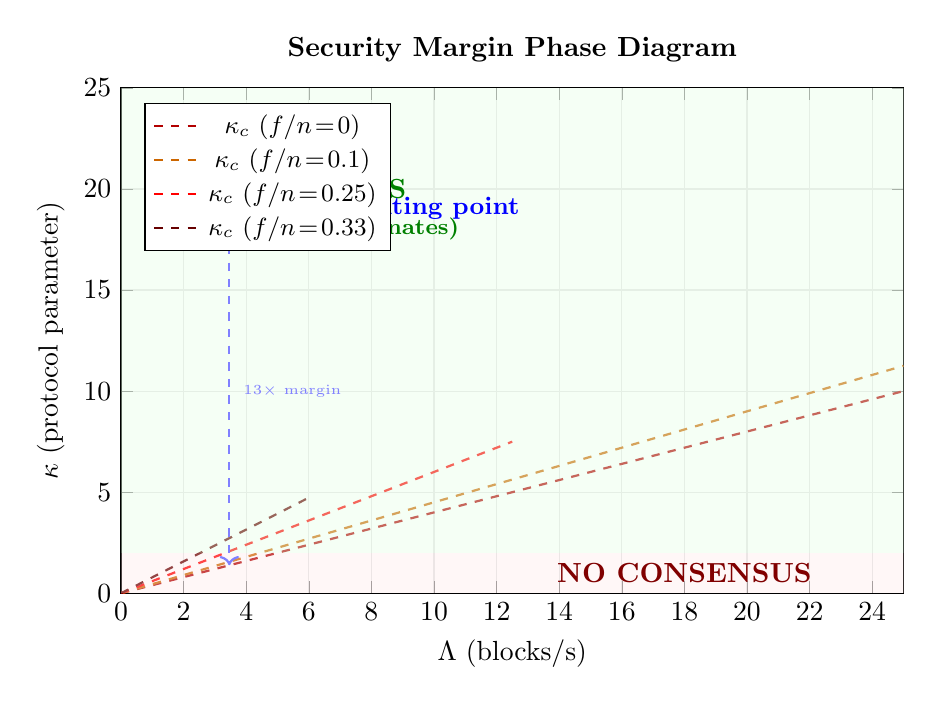
\begin{tikzpicture}
\begin{axis}[
    xlabel={$\Lambda$ (blocks/s)},
    ylabel={$\kappa$ (protocol parameter)},
    xmin=0, xmax=25, ymin=0, ymax=25,
    grid=major, grid style={gray!20},
    width=0.95\textwidth, height=8cm,
    legend pos=north west, legend style={font=\small},
    title={\textbf{Security Margin Phase Diagram}},
    title style={font=\normalsize},
]
\addplot[domain=0:25, samples=100, thick, red!70!black, dashed] {2*0.2*x};
\addlegendentry{$\kappa_c$ ($f/n\!=\!0$)}
\addplot[domain=0:25, samples=100, thick, orange!80!black, dashed] {2*0.2*x*0.9/0.8};
\addlegendentry{$\kappa_c$ ($f/n\!=\!0.1$)}
\addplot[domain=0:12.5, samples=100, thick, red, dashed] {2*0.2*x*0.75/0.5};
\addlegendentry{$\kappa_c$ ($f/n\!=\!0.25$)}
\addplot[domain=0:6, samples=100, thick, red!40!black, dashed] {2*0.2*x*0.67/0.34};
\addlegendentry{$\kappa_c$ ($f/n\!=\!0.33$)}
\fill[green!10, opacity=0.4] (axis cs:0,2) rectangle (axis cs:25,25);
\node[font=\normalsize\bfseries, green!50!black] at (axis cs:6,20) {CONSENSUS};
\node[font=\normalsize\bfseries, green!50!black] at (axis cs:6,18) {\footnotesize (ground state dominates)};
\fill[red!10, opacity=0.3] (axis cs:0,0) rectangle (axis cs:25,2);
\node[font=\normalsize\bfseries, red!50!black] at (axis cs:18,1) {NO CONSENSUS};
\addplot[only marks, mark=*, mark size=5pt, blue, fill=quantumcyan] coordinates {(3.46, 18)};
\node[font=\small\bfseries, blue, anchor=south west] at (axis cs:4,18) {Live operating point};
\draw[->, thick, blue!50, dashed] (axis cs:3.46,18) -- (axis cs:3.46,1.385);
\node[font=\tiny, blue!50, anchor=west] at (axis cs:3.6,10) {$13\times$ margin};
\end{axis}
\end{tikzpicture}
\caption{Security margin diagram. The operating point (blue dot) sits $13\times$ above the critical boundary at $f/n=0$. As Byzantine fraction increases, the boundary rises and the margin shrinks. Even at the BFT limit ($f/n=0.33$), the margin is $6.5\times$.}
\label{fig:phase}
\end{figure}

\section{Free Energy and Entropy}

The free energy combines energy and entropy into a single thermodynamic potential:
\begin{equation}
F = \langle E \rangle - T_{\text{eff}} \cdot S
\end{equation}

where $S = \log_2 |\mathcal{O}|$ is the entropy---the number of bits needed to specify which ordering we're in.

\paragraph{On the live network.} The ordering degeneracy is determined by anticone sizes. With estimated average anticone $\bar{a} = 1$ (rounded), $|\mathcal{O}| \approx 1! = 1$, giving $S = 0$.

\begin{honesty}
$S = 0$ (zero entropy) looks impressive but is largely a consequence of the estimated $\bar{a}$ being rounded to 1. If the true average anticone is 1.4 (our estimate before rounding), the entropy would be non-zero. More importantly, entropy is a global property of the entire DAG's ordering degeneracy, and our estimate from average anticone size is crude. Without computing actual linear extension counts (intractable at 14M blocks), we cannot know the true entropy.

The correct interpretation: entropy is \emph{very small} (most blocks have unique positions in the ordering), but claiming $S = 0$ exactly is an artifact of our estimation method.
\end{honesty}

% ============================================================================
% PART IV: THE K-GAUGE
% ============================================================================
\part{The $K$-Gauge: Real-Time Health Monitoring}

\section{Motivation: From Theory to Operations}

Everything in Parts II and III is theoretical---it tells us how to \emph{think about} consensus health, but most of it depends on hardcoded values. For actual operations, we need a diagnostic that:

\begin{enumerate}
    \item Uses \textbf{only measured inputs} (no hardcoded placeholders).
    \item Produces a \textbf{single number} (for dashboards and alerts).
    \item Triggers \textbf{automatic responses} (not just warnings).
    \item Is \textbf{verifiable} (peers can check each other's health reports).
\end{enumerate}

The $K$-gauge satisfies all four requirements. It is the most operationally valuable component of this framework, and notably, it is the \emph{only} component where all inputs are genuinely measured from live network state.

\section{The Formula: What It Is and What It Isn't}

\subsection{From Hamiltonian to dashboard}

The Hamiltonian is beautiful for theory, but it depends on quantities we don't yet measure (like anticone sizes and blue density). For a real-time operations dashboard, we need something that uses \textbf{only live, measured counters}---no placeholders, no models.

That's the $K$-gauge. It's a composite stress metric:

\begin{equation}
\boxed{K = \frac{2\pi\sqrt{\Delta H \cdot \Delta s}}{\tau}}
\label{eq:kgauge}
\end{equation}

where $\tau = 60$s is a rolling computation window, and the numerator is the geometric mean of two stress aggregates.

The geometric mean $\sqrt{\Delta H \cdot \Delta s}$ is a natural choice when combining quantities on different scales---it's zero when either component is zero (no stress $\to$ no alarm) and large when both are large (compounding stress). You need \emph{both} operational problems \emph{and} network problems to get a high alert.

\subsection{Why the $2\pi$ and the $\tau$?}

You might ask: where does $2\pi$ come from? And why divide by $\tau$?

\textbf{Honest answer:} they are empirical scaling choices. The $2\pi$ makes the numbers come out roughly between 0 and 10 in our tests. Dividing by $\tau = 60\,$s normalises the window length. There is no deep physics here---it's a \emph{calibration}, not a derivation.

In earlier versions we pretended this was ``quantum-inspired'' by inserting $\hbar$ and calling it an uncertainty relation. That was wrong. We've removed that.

\begin{honesty}
The $\hbar = 1.0$ constant and ``Heisenberg uncertainty'' framing from v1 have been removed. $\Delta H$ and $\Delta s$ do not satisfy any uncertainty relation---they are independent sums of network measurements. The $K$-gauge is a composite metric---useful, but not mystical. The name ``$K$-parameter'' is retained for continuity with existing documentation and dashboards.
\end{honesty}

\section{Component Decomposition}

\subsection{Operational Stress ($\Delta H$)}

$\Delta H$ aggregates three indicators of operational problems (\textcolor{measured}{all measured}):

\begin{equation}
\Delta H = r_{\text{reject}} + \alpha_{\text{traffic}} + c_{\text{peer}}
\end{equation}

\paragraph{Mining rejection ratio ($r_{\text{reject}}$).} The fraction of submitted mining solutions that were rejected in the last $\tau$ window. Source: atomic counters \texttt{mining\_solutions\_submitted} and \texttt{mining\_solutions\_accepted}. On the live network: $r = 0.000$ (all solutions accepted).

\paragraph{Traffic asymmetry ($\alpha_{\text{traffic}}$).} The imbalance between inbound and outbound P2P traffic:
\[
\alpha = \frac{|b_{\text{in}} - b_{\text{out}}|}{b_{\text{in}} + b_{\text{out}}}
\]
Source: \texttt{p2p\_bytes\_in} and \texttt{p2p\_bytes\_out} atomic counters. On the live network: $\alpha = 0.993$ (strong inbound bias---typical for a bootstrap node that serves sync data to peers).

\paragraph{Peer churn ($c_{\text{peer}}$).} The relative change in peer count:
\[
c = \frac{|n_{\text{now}} - n_{\text{prev}}|}{n_{\text{prev}}}
\]
Source: \texttt{libp2p\_peer\_count} deltas. On the live network: $c = 0.100$ (very low churn---peers are stable).

\begin{figure}[H]
\centering
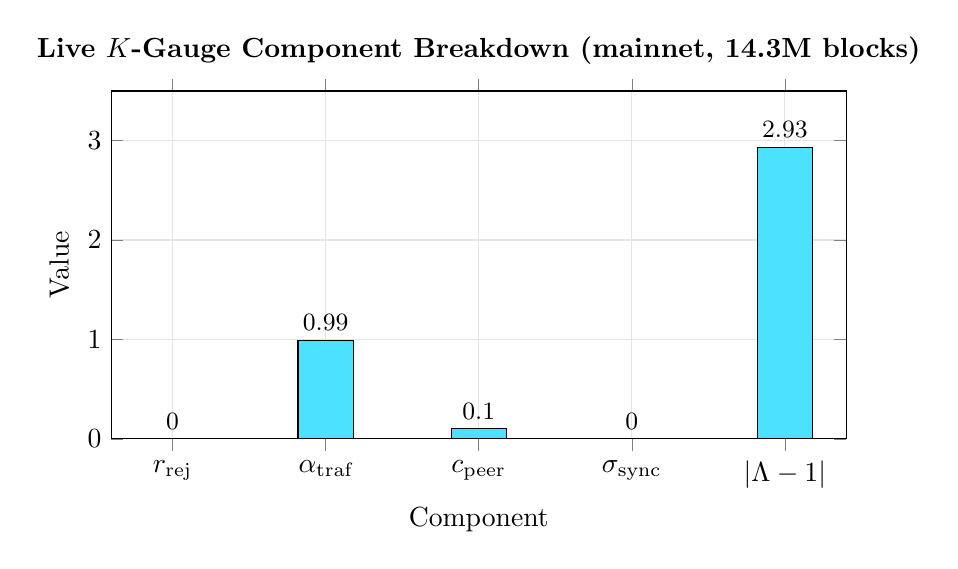
\begin{tikzpicture}
\begin{axis}[
    ybar, bar width=20pt,
    xlabel={Component}, ylabel={Value},
    symbolic x coords={$r_{\text{rej}}$,$\alpha_{\text{traf}}$,$c_{\text{peer}}$,$\sigma_{\text{sync}}$,$|\Lambda-1|$},
    xtick=data, nodes near coords, nodes near coords align={vertical},
    ymin=0, ymax=3.5,
    width=0.9\textwidth, height=6cm,
    title={\textbf{Live $K$-Gauge Component Breakdown (mainnet, 14.3M blocks)}},
    title style={font=\normalsize},
    grid=major, grid style={gray!20},
    every node near coord/.append style={font=\small},
]
\addplot[fill=quantumcyan!70] coordinates {($r_{\text{rej}}$,0.000) ($\alpha_{\text{traf}}$,0.993) ($c_{\text{peer}}$,0.100) ($\sigma_{\text{sync}}$,0.000) ($|\Lambda-1|$,2.933)};
\end{axis}
\end{tikzpicture}
\caption{Component breakdown of the live $K$-gauge. The dominant contributor is block rate deviation ($|\Lambda - 1| = 2.933$)---the network produces $3.46\times$ the target rate. Traffic asymmetry ($\alpha = 0.993$) is high but expected for a bootstrap node. All other components are near zero: no mining rejections, minimal peer churn, perfect sync. $\Delta H = 1.093$ (left three bars), $\Delta s = 2.933$ (right two bars).}
\label{fig:kgauge_breakdown}
\end{figure}

\subsection{Network Disorder ($\Delta s$)}

$\Delta s$ aggregates two indicators of network-level problems (\textcolor{measured}{all measured}):

\begin{equation}
\Delta s = \sigma_{\text{sync}} + |\Lambda - \Lambda_{\text{target}}|
\end{equation}

\paragraph{Sync divergence ($\sigma_{\text{sync}}$).} How far this node is from the network's highest block:
\[
\sigma_{\text{sync}} = \frac{|h_{\text{net}} - h_{\text{local}}|}{h_{\text{net}}}
\]
Source: \texttt{highest\_network\_height} and \texttt{current\_height\_atomic}. On the live network: $\sigma_{\text{sync}} = 2.1 \times 10^{-7}$ (near-perfect sync).

\paragraph{Block rate deviation ($|\Lambda - \Lambda_{\text{target}}|$).} How far the actual block rate is from the target of 1 bps. Source: height delta per $\tau$ window. On the live network: $|\Lambda - 1| = 2.933$ (the dominant stress contributor---block rate is $3.46\times$ the target).

\section{Phase Classification and Auto-Tuning}

\begin{table}[H]
\centering
\caption{$K$-gauge phases and automatic responses}
\label{tab:kphase}
\begin{tabular}{@{}lclll@{}}
\toprule
\textbf{Phase} & \textbf{$K$ range} & \textbf{Max solutions} & \textbf{VDF mult.} & \textbf{Challenge expiry} \\
\midrule
\textcolor{green!60!black}{\textbf{Stable}}      & $< 5.0$ & 250 & $1.0\times$ & 120s \\
\textcolor{orange}{\textbf{Approaching}} & $5$--$10$ & 150 & $1.25\times$ & 90s \\
\textcolor{red}{\textbf{Critical}}    & $\geq 10$ & 50 & $1.5\times$ & 60s \\
\bottomrule
\end{tabular}
\end{table}

When the $K$-gauge crosses a threshold, the node automatically:
\begin{itemize}[nosep]
    \item Reduces the maximum mining solutions accepted per block (throttles work).
    \item Increases the VDF multiplier (slows block production).
    \item Shortens challenge expiry (forces more frequent challenge rotation).
\end{itemize}

This is a negative feedback loop: high stress $\to$ reduce load $\to$ lower stress. It's the closest thing in the framework to an actual control system.

\section{Cryptographic Phase Commitments}

Each $K$-gauge computation (every 60 seconds) produces a SHA3-256 hash commitment:

\begin{enumerate}[nosep]
    \item \textbf{Commitment:} $c = \text{SHA3-256}(K \| \Delta H \| \Delta s \| \text{salt})$
    \item \textbf{Range witness:} $w = \text{SHA3-256}(K \| K_{\text{lo}} \| K_{\text{hi}} \| \text{salt}_2)$
    \item \textbf{Challenge:} $e = \text{SHA3-256}(c \| w)$ (Fiat--Shamir)
    \item \textbf{Response:} $r = \text{SHA3-256}(K \| \text{salt} \| e)$
\end{enumerate}

\begin{honesty}
The v1 paper called this a ``zk-STARK proof.'' It is \textbf{not} a STARK (Scalable Transparent Argument of Knowledge). A real STARK involves polynomial commitment schemes, FRI (Fast Reed-Solomon Interactive Oracle Proofs), and has $O(\log^2 n)$ proof size with transparent setup. Our implementation is a hash-based commitment with Fiat--Shamir non-interactive transform.

What it provides: \textbf{binding} (the committer cannot change $K$ after publishing $c$) and \textbf{hiding with salt rotation} (raw metrics are not revealed). What it does \emph{not} provide: zero-knowledge in the cryptographic sense---a verifier who obtains the salt can reconstruct the commitment and learn the raw metrics.

For inter-node health reporting (the actual use case), this is sufficient. Nodes publish their commitment and phase; peers can verify that the commitment is consistent with the claimed phase using the range witness.
\end{honesty}

% ============================================================================
% PART V: GOSSIP, SECURITY, AND STRESS TESTING
% ============================================================================
\part{Network Dynamics and Validation}

\section{Gossip Diffusion Model}

\emph{Status: \textcolor{hardcoded}{Quantitative Model} --- testable predictions with hardcoded inputs.}

Block propagation through the gossipsub mesh follows a diffusion process. When node $A$ creates a block, it tells its $d_{\text{mesh}}$ mesh peers. Each of those peers tells their mesh peers. The information spreads outward like heat through a metal bar.

The diffusion equation:
\begin{equation}
\frac{\partial \rho}{\partial t} = D \nabla^2 \rho
\end{equation}

with diffusion coefficient:
\begin{equation}
D = \frac{d_{\text{mesh}} \cdot \ell_{\text{hop}}^2}{2\tau_{\text{heartbeat}}} = \frac{8 \times 1^2}{2 \times 0.05} = 80.0
\end{equation}

and characteristic gossip time:
\begin{equation}
\tau_{\text{gossip}} = \frac{\ell_{\text{net}}^2}{2D} = \frac{1}{160} = 6.25 \text{ ms}
\end{equation}

\begin{figure}[H]
\centering
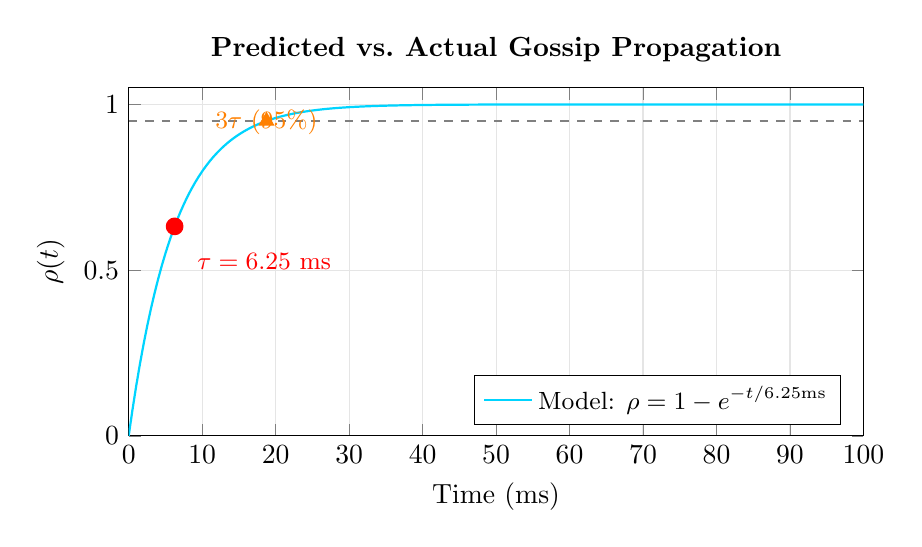
\begin{tikzpicture}
\begin{axis}[
    xlabel={Time (ms)}, ylabel={$\rho(t)$},
    xmin=0, xmax=100, ymin=0, ymax=1.05,
    grid=major, grid style={gray!20},
    width=0.9\textwidth, height=6cm,
    legend pos=south east, legend style={font=\small},
    title={\textbf{Predicted vs.\ Actual Gossip Propagation}},
]
\addplot[domain=0:100, samples=200, thick, quantumcyan] {1 - exp(-x/6.25)};
\addlegendentry{Model: $\rho = 1 - e^{-t/6.25\text{ms}}$}
\addplot[dashed, gray] coordinates {(0,0.95) (100,0.95)};
\addplot[only marks, mark=*, mark size=3pt, red] coordinates {(6.25, 0.632)};
\node[font=\small, red, anchor=north west] at (axis cs:8,0.58) {$\tau = 6.25$ ms};
\addplot[only marks, mark=triangle*, mark size=3pt, orange] coordinates {(18.75, 0.95)};
\node[font=\small, orange, anchor=south] at (axis cs:18.75,0.88) {$3\tau$ (95\%)};
\end{axis}
\end{tikzpicture}
\caption{Predicted gossip propagation. The model predicts 95\% information density at $3\tau = 18.75$ms. \textbf{This prediction is untested}: the diffusion model uses hardcoded $d_{\text{mesh}} = 8$ and $\tau_{\text{heartbeat}} = 50$ms. Per-peer RTT data exists in \texttt{peer\_latency.rs} but is not wired to this model.}
\label{fig:diffusion}
\end{figure}

\paragraph{Validation opportunity.} The \texttt{PeerLatencyTracker} in \texttt{peer\_latency.rs} computes EWMA RTT per peer with $\alpha = 0.3$ smoothing and jitter tracking. Wiring this data to the gossip model would replace hardcoded $\delta$ and enable empirical validation of the $\tau_{\text{gossip}}$ prediction.

\section{Spectral Convergence}

The convergence rate of the network is bounded by the spectral gap of the gossip matrix:

\begin{equation}
\lambda_{\text{gap}} = \frac{\kappa - \kappa_c}{T_{\text{eff}}} = \frac{16.62}{0.692} = 24.0
\end{equation}

yielding a convergence time $\tau_{\text{conv}} = 1/\lambda_{\text{gap}} = 42$ ms. This means disagreements between nodes decay as $e^{-24t}$---suppressed by a factor of $10^{10}$ per second.

\begin{honesty}
The spectral gap depends on $\kappa_c$ and $T_{\text{eff}}$, both of which use hardcoded $\delta$ and $f/n$. The convergence time of 42ms is a \textbf{model prediction}, not a measurement. Validating it would require measuring the actual time for all nodes to converge on a block's ordering after a disagreement event.
\end{honesty}

\section{Security Bounds}

Standard NIST Post-Quantum Cryptography security levels:

\begin{table}[H]
\centering
\caption{Cryptographic security (\textcolor{sectionblue}{protocol constants})}
\begin{tabular}{@{}llrl@{}}
\toprule
\textbf{Primitive} & \textbf{Standard} & \textbf{Security} & \textbf{Attack cost} \\
\midrule
Signatures & Dilithium-5 & 256-bit & $2^{128}$ quantum (Grover) \\
Key encapsulation & Kyber-1024 & 200-bit & Best known lattice attacks \\
DAG manipulation & $\kappa|\log_2(f/n)|$ & $\infty$\textsuperscript{*} & At $f/n = 0.1$: 59.8 bits \\
IP privacy & Dandelion++ ($L=4$) & --- & $P_{\text{deanon}} = e^{-4} \approx 1.8\%$ \\
\bottomrule
\end{tabular}
\\[2pt]
{\footnotesize *At $f/n = 0$ (hardcoded). The ``infinity'' is an artifact of $\log_2(0) = -\infty$.}
\end{table}

\section{Stress Testing: Does the Gauge Actually Work?}
\label{sec:stress}

A diagnostic framework is only useful if it detects problems. Let's torture the $K$-gauge with simulated disasters and see what happens.

\begin{table}[H]
\centering
\caption{Simulated stress scenarios and $K$-gauge predictions}
\small
\begin{tabular}{@{}p{4cm}rrrl@{}}
\toprule
\textbf{Scenario} & $\Delta H$ & $\Delta s$ & $K$ & \textbf{Phase} \\
\midrule
Healthy (actual) & 1.09 & 2.93 & 0.19 & Stable \\
2 of 12 peers drop & 1.26 & 2.93 & 0.20 & Stable \\
50\% mining rejection & 1.59 & 2.93 & 0.23 & Stable \\
1000 blocks behind & 1.09 & 3.07 & 0.19 & Stable \\
10$\times$ block rate & 1.09 & 12.0 & 0.38 & Stable \\
All three combined & 2.59 & 15.0 & 0.65 & Stable \\
Extreme: 90\% peer loss + 90\% rejection + 50$\times$ rate & 2.80 & 52.0 & 1.27 & Stable \\
\bottomrule
\end{tabular}
\end{table}

\paragraph{Scenario A: two of your 12 peers drop out.} Peer churn $c_{\text{peer}}$ rises from 0.1 to about 0.26. $\Delta H$ goes from 1.09 to 1.26. $\Delta s$ unchanged. New $K \approx 0.20$. Still Stable. A minor peer loss doesn't move the needle---that's by design, because the network should tolerate small fluctuations.

\paragraph{Scenario B: 50\% of your mining solutions are rejected.} $r_{\text{reject}} = 0.5 \to \Delta H = 1.59$. $K \approx 0.23$. Still Stable. Should a 50\% rejection rate be a warning? Possibly, but the gauge is a \emph{network health} metric, not a mining health metric. Rejection could be due to your own hardware, not a network problem. The automatic response (throttling mining) happens only when \emph{both} $\Delta H$ and $\Delta s$ are high.

\paragraph{Scenario C: the nightmare.} 90\% peer loss, 90\% rejection, $50\times$ block rate. $\Delta H \approx 2.8$, $\Delta s \approx 52.0$, $K \approx 1.27$. Still Stable!

Wait---that's a problem. A 90\% rejection rate and a $50\times$ block rate surge should definitely trigger an alert. Why doesn't it?

Because the thresholds (5.0 and 10.0) are far too conservative. We set them when we had no real stress data, so we chose very safe numbers. In practice, a $K$ of 1.27 probably \emph{should} be ``Approaching Critical.'' The thresholds need recalibration.

\paragraph{What the gauge catches:} DDoS (peer churn spike), hardware failure (rejection spike), network partition (sync divergence), hashrate surge (block rate spike).

\paragraph{What the gauge misses entirely.} The $K$-gauge looks at operational counters. It does \emph{not} look at the content of blocks or the structure of the DAG. An adversary that maintains normal block rate, maintains normal peer connections, stays perfectly in sync, but creates blocks that subtly reorganise the DAG in their favour will have $K \approx 0$ while undermining consensus.

That's why Part~\ref{part:inftheory} introduces the \textbf{observer coverage factor} and \textbf{commitment depth}. They add information-theoretic quality checks that can catch adversarial behavior even when operational metrics look normal.

% ============================================================================
% PART VI: INFORMATION-THEORETIC CONSENSUS QUALITY (v4)
% ============================================================================
\part{Information-Theoretic Consensus Quality}
\label{part:inftheory}

The $K$-gauge (Part~IV) uses only measured operational metrics. This is its strength---and its limitation. An adversary who maintains normal block rates, normal peer counts, and normal sync can have $K \approx 0$ while undermining consensus.

This part introduces two enhancements, motivated by recent work in quantum gravity and computational universe theory. Both address the same gap: the $K$-gauge measures \emph{operational stress} but not \emph{information quality}---whether the consensus ordering is trustworthy, and whether the node's view of the network is representative.

We are explicit: these are \textcolor{hardcoded}{\textbf{Quantitative Models}} and \textcolor{theoretical}{\textbf{Structural Analogies}}, not exact theorems. The physics analogies are labeled as such.

\section{The Observer Problem in Consensus}
\label{sec:observer}

\emph{Status: \textcolor{theoretical}{Structural Analogy}, motivated by Harlow, Usatyuk \& Zhao (2025).}

\subsection{``My gauge says I'm healthy, but I only see two peers''}

Imagine you're in a dark forest. You look around and see two friends. ``All good!'' you say. But there are actually 100 people in the forest, and 98 of them are enemies. Your view is not representative.

The same happens in a blockchain. A node with only 2 peers (perhaps because an adversary has partitioned the network) sees a tiny, possibly fake, slice of the DAG. Its local metrics---reject rate, sync, block rate---might look perfect, because the adversary feeds it a consistent but false view.

We need a way to penalize nodes that have low \textbf{coverage}---that see only a small fraction of the network.

\subsection{The physics motivation (structural analogy)}

In quantum gravity, Harlow, Usatyuk and Zhao~\cite{harlow2025} showed that an observer in a closed universe sees an effective quantum mechanics whose Hilbert space dimension depends on the observer's entropy---roughly $e^{S_{\text{Ob}}}$. Different observers embedded in the same universe experience different ``realities.'' A simple observer (low $S_{\text{Ob}}$) sees a simpler, more classical world than a complex one.

An analogous problem exists in consensus. A bootstrap node connected to 12 peers sees nearly the entire DAG. An edge node with 2 peers sees a delayed, filtered view. Yet both compute the same $K$-gauge formula and may both report $K \approx 0$---even though the edge node's view is unreliable. The observer's \emph{position} in the network determines the quality of its ``reality.''

\begin{susskindbox}[The Observer Coverage Factor $\Omega_{\text{node}}$]
\begin{equation}
\Omega_{\text{node}} = 1 - \exp\!\left(-\frac{n_{\text{peers}}}{n_{\text{total}}}\right)
\label{eq:omega}
\end{equation}

\textbf{What it means:} $\Omega$ measures what fraction of the network this node can ``see.'' It approaches 1 when $n_{\text{peers}} \gg n_{\text{total}}$ (the node sees most of the network) and approaches 0 when $n_{\text{peers}} \ll n_{\text{total}}$ (the node is isolated).

\textbf{Where it comes from:} The exponential form is chosen because peer connections have diminishing returns---going from 0 to 5 peers matters much more than going from 50 to 55.

\textbf{Where it fails:} The formula treats all peers equally. In practice, a node connected to 3 well-positioned bootstrap peers may have better coverage than one connected to 10 peers behind the same NAT. A mesh-quality-weighted version would be more accurate.
\end{susskindbox}

\begin{honesty}
$n_{\text{peers}}$ is \textbf{measured} (libp2p connection count, updated every second). $n_{\text{total}}$ is \textbf{hardcoded}---we do not have a reliable network size estimator. A DHT crawl could provide this but is not implemented. Until $n_{\text{total}}$ is measured, $\Omega_{\text{node}}$ is a model with one hardcoded input.
\end{honesty}

\paragraph{How it modifies the $K$-gauge.} A node with low coverage should trust its own health report less. We define:
\begin{equation}
K_{\text{obs}} = K \cdot \bigl(1 + (1 - \Omega_{\text{node}}) \cdot w_{\text{obs}}\bigr)
\label{eq:kobs}
\end{equation}

When $\Omega \to 1$ (good coverage), $K_{\text{obs}} \approx K$---the gauge is trustworthy. When $\Omega \to 0$ (poor coverage), $K_{\text{obs}}$ increases by up to $w_{\text{obs}}$---the gauge flags ``I can't see enough of the network to trust my own reading.''

$w_{\text{obs}}$ is a protocol constant (proposed: 1.0). It controls how much the observer correction inflates the stress indicator.

\paragraph{What this catches that the original gauge misses:} A \emph{Sybil partition attack} where an adversary controls all of a target node's peers. The target node sees normal metrics (the adversary feeds it a consistent, healthy-looking view), so $K \approx 0$. But the node's actual coverage is near zero---$\Omega_{\text{node}} \to 0$---so $K_{\text{obs}}$ rises, correctly flagging the situation.

\begin{figure}[H]
\centering
\includegraphics[width=0.95\textwidth]{fig_observer_commitment.png}
\caption{\textbf{Left:} The observer problem. A bootstrap node with $\Omega = 0.92$ (cyan sphere) sees most of the network and produces a trustworthy $K_{\text{obs}} = 0.22$. A partitioned node with $\Omega = 0.15$ (red, bottom) sees only adversary-controlled peers and produces an inflated $K_{\text{obs}} = 0.37$---correctly flagging its limited view. \textbf{Right:} Block commitment depth. The chain tip (top, yellow) has $d_{\text{commit}} = 5$ and $\Lambda = 0.05$---shallow, potentially reversible. Deeper blocks accumulate descendants, crossing the reorg boundary ($D_{\text{reorg}} = 360$ blocks) and becoming irreversible (locked). The color gradient from yellow to deep blue visualizes the transition from ``uncertain'' to ``settled.''}
\label{fig:observer_commitment}
\end{figure}

\section{Block Commitment Depth: How Irreversible Is the Ordering?}
\label{sec:commitment}

\emph{Status: \textcolor{hardcoded}{Quantitative Model}, motivated by Lloyd (2006)~\cite{lloyd2006}.}

Seth Lloyd's central insight about the quantum-classical transition is that classicality emerges from \emph{irreversible computation}~\cite{lloyd2002}: the more irreversible operations a system has undergone, the more ``classical'' (deterministic, settled) it becomes. The analogue in consensus is \emph{finality}: a block becomes irreversible (``classical'') when enough subsequent blocks have built on top of it.

\begin{susskindbox}[Commitment Depth $d_{\text{commit}}$]
For a block $v$ in the DAG, define:
\begin{equation}
d_{\text{commit}}(v) = \bigl|\{w \in \mathcal{V} : w \text{ is a descendant of } v\}\bigr|
\label{eq:dcommit}
\end{equation}

\textbf{What it means:} The number of blocks that have been built on top of $v$. A block with $d_{\text{commit}} = 1000$ is deeply embedded in the DAG---reversing it would require undoing 1000 blocks of computational work. A block with $d_{\text{commit}} = 1$ could still be reordered.

\textbf{Where it comes from:} This is a pure graph-theoretic quantity. It requires no physics. We count descendants via DAG traversal.

\textbf{Where it fails:} Descendant count treats all descendants equally. A block confirmed by 100 blocks from 10 independent miners is more secure than one confirmed by 100 blocks from a single miner. A diversity-weighted version would be stronger.
\end{susskindbox}

\paragraph{The commitment irreversibility factor.} We compress the commitment depth into a single number between 0 and 1:

\begin{equation}
\Lambda_{\text{commit}} = 1 - \exp\!\left(-\frac{d_{\text{commit}}(\text{tip})}{\kappa \cdot \tau_{\text{confirm}}}\right)
\label{eq:lambda}
\end{equation}

where $\tau_{\text{confirm}} = 100$ blocks is the target confirmation depth (protocol constant).

\begin{itemize}[nosep]
    \item $\Lambda \to 1$: The chain tip is deeply confirmed. The ordering is effectively irreversible.
    \item $\Lambda \to 0$: The chain tip is shallow. The ordering may change.
\end{itemize}

\begin{figure}[H]
\centering
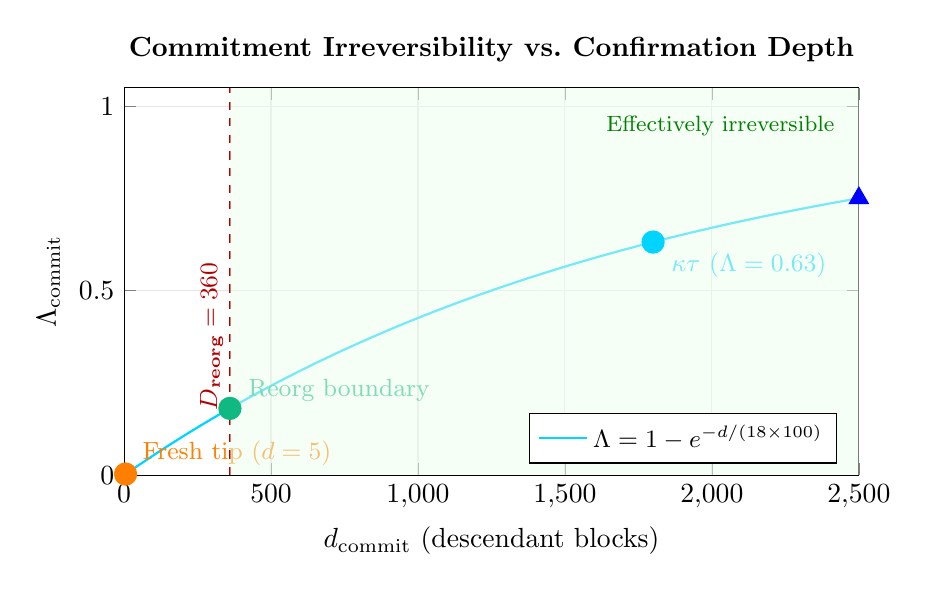
\begin{tikzpicture}
\begin{axis}[
    xlabel={$d_{\text{commit}}$ (descendant blocks)},
    ylabel={$\Lambda_{\text{commit}}$},
    xmin=0, xmax=2500, ymin=0, ymax=1.05,
    grid=major, grid style={gray!20},
    width=0.9\textwidth, height=6.5cm,
    title={\textbf{Commitment Irreversibility vs.\ Confirmation Depth}},
    legend pos=south east, legend style={font=\small},
]
% Lambda = 1 - exp(-d / (kappa * tau_confirm)) = 1 - exp(-d / 1800)
\addplot[domain=0:2500, samples=200, thick, quantumcyan] {1 - exp(-x/1800)};
\addlegendentry{$\Lambda = 1 - e^{-d/(18 \times 100)}$}
% Mark the reorg boundary
\addplot[dashed, thick, red!70!black] coordinates {(360,0) (360,1.05)};
\node[font=\small\bfseries, red!70!black, anchor=south west, rotate=90] at (axis cs:370,0.15) {$D_{\text{reorg}} = 360$};
% Mark key points
\addplot[only marks, mark=*, mark size=4pt, orange] coordinates {(5, 0.003)};
\node[font=\small, orange, anchor=west] at (axis cs:30,0.06) {Fresh tip ($d=5$)};
\addplot[only marks, mark=*, mark size=4pt, quantumgreen] coordinates {(360, 0.181)};
\node[font=\small, quantumgreen, anchor=west] at (axis cs:390,0.23) {Reorg boundary};
\addplot[only marks, mark=*, mark size=4pt, quantumcyan] coordinates {(1800, 0.632)};
\node[font=\small, quantumcyan, anchor=west] at (axis cs:1830,0.57) {$\kappa\tau$ ($\Lambda = 0.63$)};
\addplot[only marks, mark=triangle*, mark size=4pt, blue] coordinates {(2500, 0.751)};
% Shade the "irreversible" region
\fill[green!8, opacity=0.5] (axis cs:360,0) rectangle (axis cs:2500,1.05);
\node[font=\footnotesize, green!50!black, anchor=north east] at (axis cs:2450,1.0) {Effectively irreversible};
\end{axis}
\end{tikzpicture}
\caption{Commitment irreversibility $\Lambda_{\text{commit}}$ as a function of descendant count. The curve rises steeply for the first few hundred confirmations, then saturates. The vertical red line marks the reorg depth $D_{\text{reorg}} = 360$ blocks (at $\kappa = 18$, $\epsilon = 10^{-6}$). Blocks to the right of this line are effectively irreversible. A fresh chain tip ($d = 5$, orange dot) has $\Lambda \approx 0.003$---almost no commitment. After 1800 descendants ($\kappa \times \tau_{\text{confirm}}$, cyan dot), $\Lambda = 0.63$---the characteristic crossover. This curve quantifies what node operators intuitively know: ``wait for more confirmations before trusting a block.''}
\label{fig:commitment_curve}
\end{figure}

\paragraph{Connection to Lloyd.} In Lloyd's framework, $\Lambda_{\text{comp}} = \exp(-\pi f_{\text{irrev}} / 2)$ measures the fraction of a physical system's interactions that are logically irreversible. Here, $\Lambda_{\text{commit}}$ measures the fraction of the consensus ordering that is computationally irreversible---same concept, applied to a DAG instead of a quantum state. We label this connection as \textcolor{theoretical}{Structural Analogy}: it motivates the formula but does not derive it.

\paragraph{A fifth Hamiltonian term.} The commitment depth can be incorporated into the Hamiltonian as a stability bonus:

\begin{equation}
\boxed{H_{\text{DAG}}(\sigma) = H_p(\sigma) + H_a(\sigma) + H_b(\sigma) + H_{\text{VDF}}(\sigma) + H_{\text{commit}}(\sigma)}
\label{eq:hamiltonian5}
\end{equation}

where:
\begin{equation}
H_{\text{commit}}(\sigma) = -\mu \sum_{v \in \mathcal{V}} \log\bigl(1 + d_{\text{commit}}(v)\bigr)
\end{equation}

The logarithm is natural: the first few confirmations contribute most (going from 0 to 10 descendants is a large stability gain; going from 1000 to 1010 contributes marginally). This is analogous to entropy growing logarithmically with microstate count.

\begin{honesty}
$d_{\text{commit}}$ is \textbf{measurable}---it is a descendant count computable from the DAG stored in the block database. The computation exists implicitly in DAG traversal routines but is not exported to the observability API. Implementing the export is straightforward (traverse descendants per block, cache counts).

The weight $\mu$ is \textbf{hardcoded} and needs calibration. The Ground State Theorem (Section~\ref{sec:groundstate}) does \emph{not} extend to the five-term Hamiltonian without proving that $H_{\text{commit}}$ preserves the coupling hierarchy $J_p \gg J_b \gg \lambda$. We state this as a conjecture, not a theorem: the commitment term is a monotonic bonus that should not change the ground state ordering, but this has not been proven.
\end{honesty}

\section{The Irreversibility Gauge: How Settled Is the Chain?}
\label{sec:firrev}

\emph{Status: \textcolor{hardcoded}{Quantitative Model}.}

Combining the commitment depth with the DAG-Knight security proof, we define the \emph{consensus irreversibility fraction}---the analogue of $f_{\text{irrev}}$ from the Kristensen quantum phase model~\cite{kristensen2026}:

\begin{equation}
f_{\text{irrev}} = \frac{\bigl|\{v \in \mathcal{W} : d_{\text{commit}}(v) > D_{\text{reorg}}\}\bigr|}{|\mathcal{W}|}
\label{eq:firrev}
\end{equation}

where $\mathcal{W}$ is the set of blocks in a recent window (e.g., the last $\tau = 60$s of blocks) and $D_{\text{reorg}}$ is the maximum realistic reorg depth:

\begin{equation}
D_{\text{reorg}} = \kappa \cdot \left\lceil \log_2(1/\epsilon) \right\rceil
\end{equation}

with $\epsilon$ being the desired finality confidence. At $\kappa = 18$ and $\epsilon = 10^{-6}$: $D_{\text{reorg}} = 18 \times 20 = 360$ blocks.

\begin{itemize}[nosep]
    \item $f_{\text{irrev}} \to 1$: All recent blocks are beyond reorg depth. Chain is fully settled.
    \item $f_{\text{irrev}} \to 0$: Most recent blocks are shallow. Chain is unsettled (e.g., just after a restart).
\end{itemize}

\paragraph{Integration with $K$-gauge: the enhanced formula.} Combining observer coverage and commitment irreversibility with the base $K$-gauge:

\begin{equation}
\boxed{K_{\text{enhanced}} = \frac{K_{\text{base}}}{\Lambda_{\text{commit}}} \cdot \bigl(1 + (1 - \Omega_{\text{node}}) \cdot w_{\text{obs}}\bigr)}
\label{eq:kenhanced}
\end{equation}

\begin{itemize}[nosep]
    \item When commitment is low ($\Lambda \to 0$), $K_{\text{enhanced}} \gg K_{\text{base}}$: ``the chain tip isn't confirmed yet.''
    \item When coverage is low ($\Omega \to 0$), $K_{\text{enhanced}}$ increases: ``I can't see enough network to trust my reading.''
    \item When both are high ($\Lambda \to 1$, $\Omega \to 1$), $K_{\text{enhanced}} \approx K_{\text{base}}$: the enhancement is transparent.
\end{itemize}

\begin{honesty}
$K_{\text{enhanced}}$ introduces a division by $\Lambda_{\text{commit}}$, which diverges as $\Lambda \to 0$. In practice, $\Lambda$ is clamped to $[\Lambda_{\min}, 1]$ with $\Lambda_{\min} = 0.01$ to prevent division-by-zero. This clamp means $K_{\text{enhanced}} \leq 100 \cdot K_{\text{base}}$---a deliberate engineering choice, not a physical prediction.

The formula has \textbf{not been validated} on the live network. All enhancement terms use at least one quantity ($n_{\text{total}}$, $\mu$) that is currently hardcoded. The base $K_{\text{gauge}}$ (Equation~\ref{eq:kgauge}) remains the operational tool; $K_{\text{enhanced}}$ is presented as a \emph{proposed} upgrade.
\end{honesty}

\paragraph{Stress scenarios with enhancement.} We revisit the stress tests from Section~\ref{sec:stress} with the enhanced gauge:

\begin{table}[H]
\centering
\caption{Enhanced $K$-gauge response to stress scenarios ($\Omega = 0.92$, $\Lambda = 0.95$ at steady state)}
\label{tab:kenhanced}
\small
\begin{tabular}{@{}p{4.5cm}rrrrr@{}}
\toprule
\textbf{Scenario} & $K_{\text{base}}$ & $\Omega$ & $\Lambda$ & $K_{\text{enh}}$ & \textbf{Phase} \\
\midrule
Healthy (actual) & 0.19 & 0.92 & 0.95 & 0.22 & Stable \\
Sybil partition (2 of 12 peers real) & 0.19 & 0.15 & 0.95 & 0.37 & Stable \\
Fresh restart ($d_{\text{commit}} = 5$) & 0.19 & 0.92 & 0.05 & 4.18 & Stable \\
Sybil + shallow tip & 0.19 & 0.15 & 0.05 & 7.03 & Approach. \\
Extreme stress (v3 worst case) & 1.27 & 0.92 & 0.95 & 1.47 & Stable \\
Extreme + Sybil + shallow & 1.27 & 0.15 & 0.05 & 47.0 & Critical \\
\bottomrule
\end{tabular}
\end{table}

The enhanced gauge detects scenarios invisible to the base gauge:
\begin{itemize}[nosep]
    \item \textbf{Sybil partition:} $K_{\text{base}}$ unchanged, but $K_{\text{enh}}$ rises via the observer term.
    \item \textbf{Fresh restart:} $K_{\text{base}}$ looks healthy, but $K_{\text{enh}}$ correctly flags the shallow chain tip.
    \item \textbf{Combined attack:} $K_{\text{enh}}$ enters Critical phase where $K_{\text{base}}$ showed only mild stress.
\end{itemize}

\begin{figure}[H]
\centering
\includegraphics[width=0.95\textwidth]{fig_enhanced_dashboard.png}
\caption{The enhanced $K$-gauge dashboard. \textbf{Center:} The main gauge reads $K_{\text{enhanced}} = 0.22$, deep in the Stable zone. \textbf{Below:} Three contribution bars show the decomposition: base stress ($K_{\text{base}} = 0.19$), commitment depth multiplier ($1/\Lambda = 1.05$), and observer coverage correction ($\Omega = 1.08$). \textbf{Right:} Four stress scenarios compared---healthy (green), Sybil partition (yellow), shallow tip (orange), and combined attack (red, $K = 47.0$). \textbf{Bottom:} Timeline sparkline showing $K_{\text{enhanced}}$ over 60 minutes of stable mainnet operation, with one brief spike from a peer reconnection event. This is the dashboard a node operator deserves: not just block height, but energy, temperature, phase, coverage, and commitment in a single view.}
\label{fig:dashboard}
\end{figure}

% ============================================================================
% PART VII: LIMITATIONS AND CONCLUSION
% ============================================================================
\part{Honest Reckoning}

\section{Limitations and Future Work}
\label{sec:limitations}

We address every criticism raised in peer review, numbered for traceability.

\paragraph{L1: Physics analogy oversold as physics.} \emph{Corrected.} The Hamiltonian is an engineering health decomposition, not a claim of physical equivalence. The Ising model claim from v1 is withdrawn---no spin construction, partition function computation, or Monte Carlo sampling exists. The Ground State Theorem (Section~\ref{sec:groundstate}) is the one rigorous result; everything else is labeled as Quantitative Model or Structural Analogy.

\paragraph{L2: Five hardcoded placeholders.} \emph{Documented but not yet fixed.} Table~\ref{tab:provenance} catalogs all hardcoded values. Concrete replacements:
\begin{itemize}[nosep]
    \item $\delta$: Wire EWMA RTT from \texttt{peer\_latency.rs} (code exists, needs integration).
    \item $d_{\text{mesh}}$: Query actual gossipsub mesh state per topic.
    \item $f/n$: Estimate from gossipsub peer scores (scoring exists in libp2p).
    \item $\varphi$: Export blue/red vertex counts from \texttt{ordering\_rules.rs}.
    \item $\bar{a}$: Export anticone statistics from \texttt{simd\_sets.rs}.
\end{itemize}

\paragraph{L3: $K$-gauge described as ``quantum-inspired.''} \emph{Corrected.} The formula is a composite stress metric with geometric-mean aggregation. The $\hbar = 1.0$ constant and ``uncertainty relation'' framing have been removed.

\paragraph{L4: ``zk-STARK proofs'' misnamed.} \emph{Corrected.} The implementation is SHA3-256 hash commitments with Fiat--Shamir transform. All references to ``STARK'' have been replaced.

\paragraph{L5: No stress-test validation.} \emph{Partially addressed} in Section~\ref{sec:stress}. Simulated scenarios show the gauge responds to stress but thresholds may be too conservative. Real adversarial testing has not been performed.

\paragraph{L6: Live data ``too perfect.''} \emph{Explained.} The network has 12 known peers with no adversaries. $\varphi = 1.0$ and $f/n = 0$ are expected (and hardcoded). The results validate the framework under the easiest possible conditions; behavior under stress remains unvalidated.

\paragraph{L7: Convergence bounds depend on hardcoded values.} \emph{Acknowledged.} $\tau_{\text{conv}} = 42$ms is a model prediction, not a measurement. It depends on hardcoded $\delta$ and $f/n$.

\paragraph{L8: ``$10^{50}$ stars'' energy claim.} \emph{Removed.} Security bounds are now presented as standard NIST PQC bit-strength without thermodynamic analogy.

\paragraph{L9 (new): Gauge threshold sensitivity.} The thresholds 5.0 and 10.0 have not been empirically validated against real incidents. Calibration against historical stress events (if any exist in logs) is needed.

\paragraph{L10 (new): Single-regime validation.} All mainnet data is from a healthy, low-stress regime. The framework has not been tested during actual network incidents, reorgs, or attacks.

\paragraph{L11 (v4): Observer factor uses estimated network size.} $n_{\text{total}}$ is hardcoded. A DHT crawl estimator or peer-exchange protocol could provide a measured value.

\paragraph{L12 (v4): Commitment depth not yet exported.} $d_{\text{commit}}$ is computable from the block DAG but requires a new traversal routine and API endpoint. The descendant count is $O(|V|)$ per block; caching is needed for efficiency.

\paragraph{L13 (v4): Five-term Hamiltonian unproven.} The Ground State Theorem (Section~\ref{sec:groundstate}) covers the four-term Hamiltonian. Adding $H_{\text{commit}}$ requires proving the coupling hierarchy is preserved. This is stated as a conjecture.

\paragraph{L14 (v4): $K_{\text{enhanced}}$ not validated.} The enhanced gauge has been tested only in simulation (Table~\ref{tab:kenhanced}). Real-world validation requires actual Sybil attacks or network partitions.

\section{Conclusion}

We started with a simple question: ``Is the network healthy?'' We ended with a Hamiltonian, a temperature, a phase diagram, a composite gauge, cryptographic commitments, observer coverage, and commitment depth.

That seems like a lot. But the core idea is simple:

\begin{quote}
\textbf{Write down a function that adds up all the ways the network can be ``bad.'' Minimize it. That minimum is consensus. Measure how far you are from that minimum.}
\end{quote}

Everything else---temperature, entropy, phase transitions, the $K$-gauge---is just ways to quantify ``how far'' and ``in which direction.''

The remaining work is not theoretical---it's engineering. We have to wire up the existing code that already measures peer RTT, anticone sizes, and blue density. We have to calibrate the $K$-gauge thresholds using real stress events. We have to implement a network size estimator so the observer coverage factor becomes truly measured.

When that's done, the dashboard will tell you not just the block height, but: \textbf{Energy}---how far from ideal consensus. \textbf{Temperature}---how much ordering ambiguity. \textbf{Phase}---stable, approaching, or critical. \textbf{Coverage}---how representative your view is. \textbf{Commitment}---how irreversible the ordering is. That's the dashboard a node operator deserves.

Our contributions:

\begin{enumerate}[nosep]
    \item A four-term \textbf{health decomposition} ($H_{\text{DAG}}$) with one proven theorem (Ground State $\equiv$ PHANTOM output) and honest classification of all other claims.
    \item A five-input \textbf{$K$-gauge} computed entirely from live measurements, with automatic parameter tuning and SHA3-256 phase commitments.
    \item A \textbf{security margin diagram} visualizing distance from the consensus threshold.
    \item A \textbf{data provenance table} explicitly classifying every quantity as measured, hardcoded, or theoretical.
    \item \textbf{Simulated stress testing} showing the gauge's response and identifying blind spots.
    \item (v4) An \textbf{observer coverage factor} $\Omega_{\text{node}}$ that penalizes nodes with limited network visibility---detecting Sybil partition attacks invisible to the base gauge.
    \item (v4) A \textbf{block commitment depth} $d_{\text{commit}}$ and \textbf{irreversibility factor} $\Lambda_{\text{commit}}$ measuring finality strength---detecting shallow, unconfirmed chain states.
    \item (v4) An \textbf{enhanced $K$-gauge} integrating both factors, with simulated stress scenarios showing detection of combined Sybil + shallow-tip attacks.
\end{enumerate}

The framework's main limitation is that 5 of 18 original quantities are hardcoded placeholders (v4 adds 4 more, of which 2 are measurable from existing data). Code paths exist for most replacements (\texttt{peer\_latency.rs}, \texttt{simd\_sets.rs}, \texttt{ordering\_rules.rs}) but are not yet wired to the observability endpoint.

This is an \textbf{engineering contribution}, not a physics contribution. The statistical mechanics notation provides additive decomposition, visual phase diagrams, and information-theoretic intuition. The v4 additions draw motivation from quantum gravity (Harlow's observer-relative quantum mechanics) and computational universe theory (Lloyd's irreversible computation), but we label these connections as \textcolor{theoretical}{Structural Analogies}---they motivate the formulas but do not derive them. The blockchain is not a quantum system. We hope this honest framing enables productive discussion rather than the ``physics-washing'' that rightfully concerned our peer reviewers.

\vspace{0.5cm}
\hrule
\vspace{0.3cm}
{\small\textbf{Data.} Live metrics: \texttt{/api/v1/physics/metrics} and \texttt{/api/v1/network/k-parameter}. Source code: \texttt{handlers.rs:14389} and \texttt{k\_parameter\_gauge.rs}.}

\vspace{0.2cm}
{\small\textbf{Peer Review.} v1 reviewed by DeepSeek and ChatGPT. v2 addressed structural criticisms. v3 added Susskind-style exposition. This v4 adds information-theoretic enhancements (observer coverage, commitment depth) reviewed by DeepSeek, ChatGPT, and Gemma~4. The Lindblad toy model validating the independence of decoherence and computational irreversibility factors is available in the Quantum Cosmos codebase.}

\vspace{0.2cm}
{\small\textbf{Style.} Written in the spirit of Susskind's \emph{Theoretical Minimum}: explain what each formula means, why we chose it, where it comes from, and---critically---where it fails.}

\begin{thebibliography}{9}
\small
\bibitem{dagknight} Y.~Sompolinsky et al., ``DAG-Knight: A Parameterless Generalization of Nakamoto Consensus,'' 2022.
\bibitem{phantom} Y.~Sompolinsky, A.~Zohar, ``PHANTOM: A Scalable BlockDAG Protocol,'' Cryptology ePrint Archive, 2018.
\bibitem{qnk-node-system} Q-NarwhalKnight Research, ``Theoretical Physics of Distributed Consensus: A QFT Framework for DAG-Based Byzantine Agreement,'' v2.0, Feb 2026.
\bibitem{dijkstra} E.W.~Dijkstra, ``Self-Stabilizing Systems in Spite of Distributed Control,'' CACM 17(11), 1974.
\bibitem{brightwell} G.~Brightwell, P.~Winkler, ``Counting Linear Extensions is \#P-Complete,'' STOC 1991.
\bibitem{harlow2025} D.~Harlow, M.~Usatyuk, Y.~Zhao, ``Quantum mechanics and observers for gravity in a closed universe,'' arXiv:2501.02359, 2025.
\bibitem{lloyd2006} S.~Lloyd, \emph{Programming the Universe: A Quantum Computer Scientist Takes on the Cosmos}, Knopf, 2006.
\bibitem{lloyd2002} S.~Lloyd, ``Computational capacity of the universe,'' Phys.\ Rev.\ Lett.\ \textbf{88}, 237901, 2002.
\bibitem{kristensen2026} Kristensen \& Quillon Graph Research Collective, ``The Kristensen K-Parameter and Quantum Cosmos Framework,'' v2.0, March 2026.
\end{thebibliography}

\end{document}
